\chapter*{Справочные таблицы}\addcontentsline{toc}{chapter}{Справочные таблицы}\markright{Таблицы}

\section*{Таблица умножения от 0 до 10}

\begingroup\small\renewcommand{\arraystretch}{1.4}\setlength{\tabcolsep}{5pt}\arrayrulecolor{Teal}

\begin{center}\begin{tabular}{|c|r|r|r|r|r|r|r|r|r|r|r|}\hline

\(\times\)&0&1&2&3&4&5&6&7&8&9&10\\\hline

0&0&0&0&0&0&0&0&0&0&0&0\\\hline

1&0&1&2&3&4&5&6&7&8&9&10\\\hline

2&0&2&4&6&8&10&12&14&16&18&20\\\hline

3&0&3&6&9&12&15&18&21&24&27&30\\\hline

4&0&4&8&12&16&20&24&28&32&36&40\\\hline

5&0&5&10&15&20&25&30&35&40&45&50\\\hline

6&0&6&12&18&24&30&36&42&48&54&60\\\hline

7&0&7&14&21&28&35&42&49&56&63&70\\\hline

8&0&8&16&24&32&40&48&56&64&72&80\\\hline

9&0&9&18&27&36&45&54&63&72&81&90\\\hline

10&0&10&20&30&40&50&60&70&80&90&100\\\hline

\end{tabular}\end{center}\endgroup

\par\addvspace{5pt}\begin{lrbox}{\CatFlowBox}\begin{minipage}[t]{\linewidth}
\setlength{\parskip}{5pt}\setlength{\columnsep}{4.5mm}\setlength{\intextsep}{0pt}
\begin{wrapfigure}[11]{r}{54mm}

\includegraphics[width=54mm,height=58mm,keepaspectratio]{images/unique/art-96.png}
\end{wrapfigure}
Таблица симметрична относительно главной диагонали: это отражает коммутативность умножения \(ab=ba\). В нулевой строке стоят нули, а строка единицы повторяет заголовки столбцов. Дистрибутивность связывает соседние строки: например, \(7b=5b+2b\). Эти наблюдения позволяют восстанавливать результаты по свойствам действий и позднее узнавать те же свойства в алгебраических структурах.
\par\WFclear\end{minipage}\end{lrbox}%
\ifdim\dimexpr\ht\CatFlowBox+\dp\CatFlowBox\relax<64mm\dp\CatFlowBox=\dimexpr64mm-\ht\CatFlowBox\relax\fi%
\noindent\usebox{\CatFlowBox}\par\addvspace{5pt}
% TRIG_TABLE_START
\par\noindent\begin{minipage}{\linewidth}
\section*{Тригонометрические значения}

Углы даны в радианах. Прочерк означает, что функция в этой точке не определена.

\begingroup\renewcommand{\arraystretch}{1.5}\arrayrulecolor{Teal}\begin{center}\begin{tabular}{|c|c|c|c|}\hline\(x\)&\(\sin x\)&\(\cos x\)&\(\operatorname{tg}x\)\\[3pt]\hline

\(\displaystyle 0\)&\(\displaystyle 0\)&\(\displaystyle 1\)&\(\displaystyle 0\)\\[3pt]\hline

\(\displaystyle \frac\pi6\)&\(\displaystyle \frac12\)&\(\displaystyle \frac{\sqrt3}2\)&\(\displaystyle \frac{\sqrt3}3\)\\[3pt]\hline

\(\displaystyle \frac\pi4\)&\(\displaystyle \frac{\sqrt2}2\)&\(\displaystyle \frac{\sqrt2}2\)&\(\displaystyle 1\)\\[3pt]\hline

\(\displaystyle \frac\pi3\)&\(\displaystyle \frac{\sqrt3}2\)&\(\displaystyle \frac12\)&\(\displaystyle \sqrt3\)\\[3pt]\hline

\(\displaystyle \frac\pi2\)&\(\displaystyle 1\)&\(\displaystyle 0\)&---\\[3pt]\hline

\(\displaystyle \pi\)&\(\displaystyle 0\)&\(\displaystyle -1\)&\(\displaystyle 0\)\\[3pt]\hline

\(\displaystyle \frac{3\pi}2\)&\(\displaystyle -1\)&\(\displaystyle 0\)&---\\[3pt]\hline

\(\displaystyle 2\pi\)&\(\displaystyle 0\)&\(\displaystyle 1\)&\(\displaystyle 0\)\\[3pt]\hline

\end{tabular}\end{center}\endgroup

\end{minipage}\par

\section*{Производные базовых функций}

В тригонометрических формулах аргумент измеряется в радианах. Степенные и простые рациональные случаи разобраны в главе 20; формулы для экспоненты, логарифма, тригонометрических и обратных функций приведены для справки. Их доказательства изучаются в дальнейшем курсе анализа.

\begingroup\small\renewcommand{\arraystretch}{1.6}\arrayrulecolor{Teal}\begin{longtable}{|p{.25\linewidth}|p{.29\linewidth}|p{.36\linewidth}|}\hline\(f(x)\)&\(f'(x)\)&Условия\\[3pt]\hline\endfirsthead\hline\(f(x)\)&\(f'(x)\)&Условия\\[3pt]\hline\endhead

\(\displaystyle c\)&\(\displaystyle 0\)&\(c\) — постоянная; \(x\in\mathbb R\).\\[3pt]\hline

\(\displaystyle x\)&\(\displaystyle 1\)&\(x\in\mathbb R\).\\[3pt]\hline
\(\displaystyle x^n\)&\(\displaystyle nx^{n-1}\)&\(n\in\mathbb N\), \(n\ge2\); \(x\in\mathbb R\).\\[3pt]\hline

\(\displaystyle x^\alpha\)&\(\displaystyle \alpha x^{\alpha-1}\)&\(\alpha\in\mathbb R\) постоянна; \(x>0\).\\[3pt]\hline

\(\displaystyle \sqrt x\)&\(\displaystyle \frac1{2\sqrt x}\)&\(x>0\).\\[3pt]\hline

\(\displaystyle \frac1x\)&\(\displaystyle -\frac1{x^2}\)&\(x\ne0\).\\[3pt]\hline

\(\displaystyle e^x\)&\(\displaystyle e^x\)&\(x\in\mathbb R\).\\[3pt]\hline

\(\displaystyle a^x\)&\(\displaystyle a^x\ln a\)&\(a>0\) постоянно; \(x\in\mathbb R\).\\[3pt]\hline

\(\displaystyle \ln x\)&\(\displaystyle \frac1x\)&\(x>0\).\\[3pt]\hline

\(\displaystyle \log_a x\)&\(\displaystyle \frac1{x\ln a}\)&\(a>0\), \(a\ne1\), \(x>0\).\\[3pt]\hline

\(\displaystyle \sin x\)&\(\displaystyle \cos x\)&\(x\in\mathbb R\).\\[3pt]\hline

\(\displaystyle \cos x\)&\(\displaystyle -\sin x\)&\(x\in\mathbb R\).\\[3pt]\hline

\(\displaystyle \operatorname{tg}x\)&\(\displaystyle \frac1{\cos^2x}\)&\(\cos x\ne0\).\\[3pt]\hline

\(\displaystyle \arcsin x\)&\(\displaystyle \frac1{\sqrt{1-x^2}}\)&\(-1<x<1\).\\[3pt]\hline

\(\displaystyle \arccos x\)&\(\displaystyle -\frac1{\sqrt{1-x^2}}\)&\(-1<x<1\).\\[3pt]\hline

\(\displaystyle \operatorname{arctg}x\)&\(\displaystyle \frac1{1+x^2}\)&\(x\in\mathbb R\).\\[3pt]\hline

\(\displaystyle \operatorname{sh}x\)&\(\displaystyle \operatorname{ch}x\)&\(x\in\mathbb R\).\\[3pt]\hline

\(\displaystyle \operatorname{ch}x\)&\(\displaystyle \operatorname{sh}x\)&\(x\in\mathbb R\).\\[3pt]\hline

\end{longtable}\endgroup

\section*{Правила дифференцирования}

В точках, где \(u,v\) дифференцируемы, а \(c\) постоянно:

\[\begin{gathered}(cu)'=cu',\qquad (u+v)'=u'+v',\\(uv)'=u' v+uv',\qquad \left(\frac uv\right)'=\frac{u' v-uv'}{v^2}\quad(v\ne0).\end{gathered}\]

Для композиции дополнительно требуется дифференцируемость \(f\) в точке \(u(x)\):

\[(f\circ u)'(x)=f'(u(x))u'(x).\]

Это правило цепочки (\emph{chain rule}); оно приведено как справочное правило для дальнейшего изучения.

\par\addvspace{5pt}\begin{lrbox}{\CatFlowBox}\begin{minipage}[t]{\linewidth}
\setlength{\parskip}{5pt}\setlength{\columnsep}{4.5mm}\setlength{\intextsep}{0pt}
\begin{wrapfigure}[11]{l}{54mm}
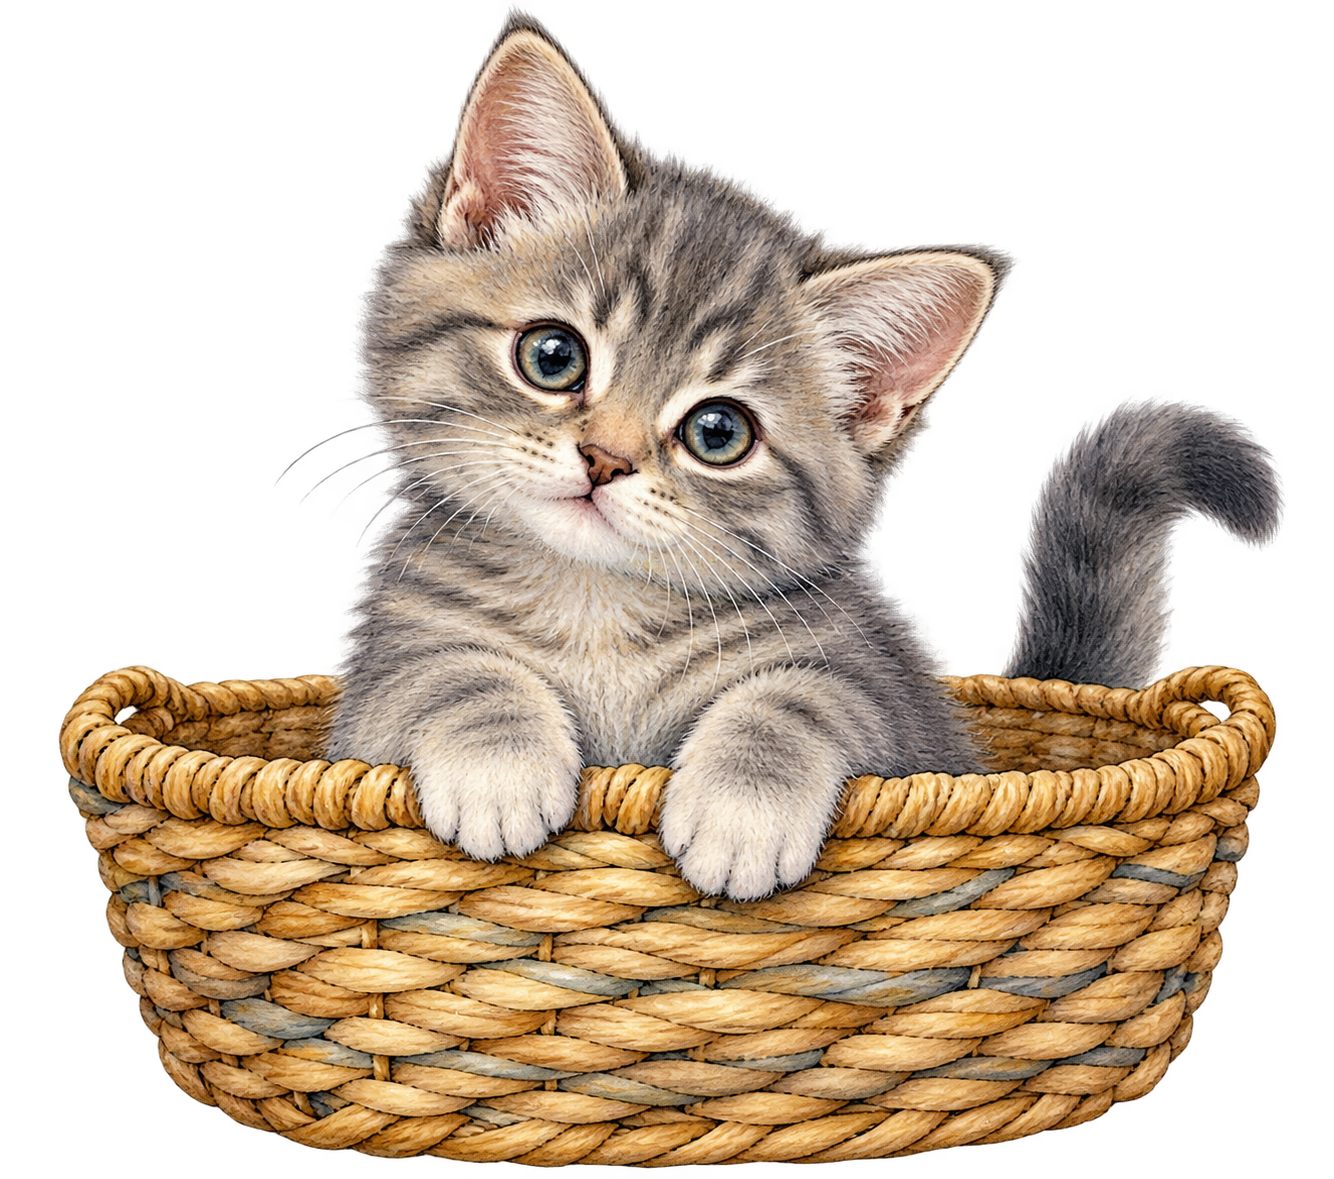
\includegraphics[width=54mm,height=58mm,keepaspectratio]{images/unique/art-97.png}
\end{wrapfigure}
Правило цепочки учитывает, что аргумент внешней функции сам меняется. Например, в \(e^{x^2}\) внешняя функция — экспонента, а внутренняя — \(u(x)=x^2\). Поэтому
\[
\left(e^{x^2}\right)'=e^{x^2}\cdot2x.
\]
Для сравнения, производная \(e^x\) равна \(e^x\): у внутреннего аргумента \(x\) производная равна \(1\). В обоих случаях применяется одно правило, меняется лишь внутренняя функция.
\par\WFclear\end{minipage}\end{lrbox}%
\ifdim\dimexpr\ht\CatFlowBox+\dp\CatFlowBox\relax<64mm\dp\CatFlowBox=\dimexpr64mm-\ht\CatFlowBox\relax\fi%
\noindent\usebox{\CatFlowBox}\par\addvspace{5pt}
\section*{Степени и логарифмы}

Для \(a,b>0\), \(r,s\in\mathbb R\):

\[a^{r+s}=a^ra^s,\qquad (a^r)^s=a^{rs},\qquad (ab)^r=a^rb^r.\]

При \(a>0\), \(a\ne1\), \(u,v>0\), \(r\in\mathbb R\):

\[\begin{gathered}\log_a(uv)=\log_a u+\log_a v,\qquad \log_a\frac uv=\log_a u-\log_a v,\\\log_a(u^r)=r\log_a u,\qquad\log_a u=\frac{\ln u}{\ln a}.\end{gathered}\]

\section*{Тригонометрические тождества}

Для действительных \(x,y\):

\[\begin{gathered}\sin^2x+\cos^2x=1,\\\sin(x\pm y)=\sin x\cos y\pm\cos x\sin y,\\\cos(x\pm y)=\cos x\cos y\mp\sin x\sin y,\\\sin2x=2\sin x\cos x,\qquad\cos2x=\cos^2x-\sin^2x.\end{gathered}\]

При определённости каждого тангенса:

\[\operatorname{tg}(x+y)=\frac{\operatorname{tg}x+\operatorname{tg}y}{1-\operatorname{tg}x\operatorname{tg}y}.\]

Знаменатель в последней формуле должен быть ненулевым.


\par\addvspace{5pt}\begin{lrbox}{\CatFlowBox}\begin{minipage}[t]{\linewidth}
\setlength{\parskip}{5pt}\setlength{\columnsep}{4.5mm}\setlength{\intextsep}{0pt}
\begin{wrapfigure}[12]{r}{54mm}

\includegraphics[width=54mm,height=58mm,keepaspectratio]{images/unique/art-98.png}
\end{wrapfigure}
Формулы сложения дают значения в новых точках через уже известные. Так, из \(\cos(\pi-x)=\cos\pi\cos x+\sin\pi\sin x\) получаем \(\cos(\pi-x)=-\cos x\). Аналогично \(\sin(\pi-x)=\sin x\). Поэтому углы \(\frac\pi6\) и \(\frac{5\pi}6\) имеют одинаковые синусы и противоположные косинусы. Это следует из тождеств для всех действительных аргументов, а не только из отдельных строк таблицы.
\par\WFclear\end{minipage}\end{lrbox}%
\ifdim\dimexpr\ht\CatFlowBox+\dp\CatFlowBox\relax<64mm\dp\CatFlowBox=\dimexpr64mm-\ht\CatFlowBox\relax\fi%
\noindent\usebox{\CatFlowBox}\par\addvspace{5pt}

